\clearpage

\section{相关理论与技术}

\subsection{AoI相关概述与通用计算框架}
在深入探讨具体的 MAC 协议之前，本节将首先对 AoI 这一核心评价指标进行详细的介绍，并利用几何分析与随机过程理论，推导出一套适用于后续各类具体退避算法的通用性能计算框架。

\subsubsection{AoI的定义与演化特性}
考虑如图\ref{fig:communication_system}所示的通信系统，该系统由一个传感器节点和一个远程接收机组成，传感器节点以速率 $\lambda$ 持续地产生数据包，产生的数据包会被放到缓冲队列中，随后服务器会以 $\mu$ 的服务速率将数据包通过无线信道发送到远程接收机。

\begin{figure}[h]
    \centering
    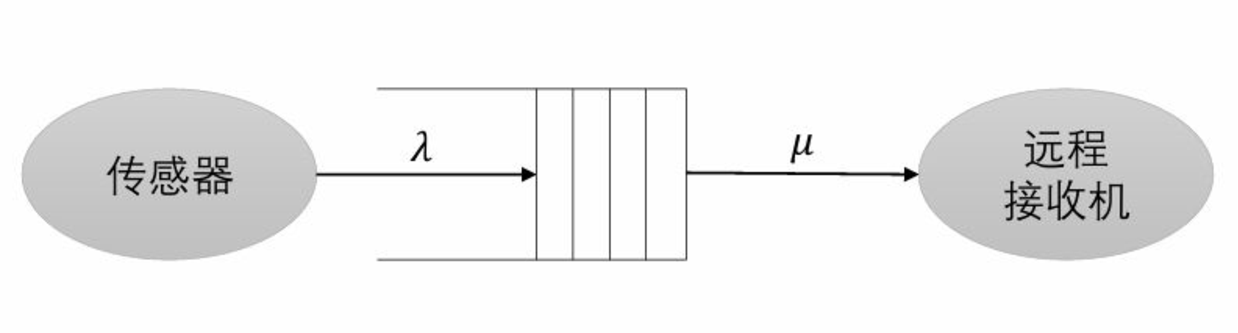
\includegraphics[width=0.8\textwidth]{figure/cp2/2.1.pdf}
    \caption{通信系统}
    \label{fig:communication_system}
\end{figure}

设 $t$ 为当前系统的观测时刻，$u(t)$为接收机在 $t$ 时刻所掌握的最新数据包的生成时间，则 AoI 为
\begin{equation}
    \Delta(t) = t - u(t)
\end{equation}
该定义直观地反映了接收机当前所拥有的状态信息的陈旧程度。随着时间 $t$ 的推移，如果接收机迟迟未收到新的状态更新，$u(t)$ 将保持不变，$\Delta(t)$ 就会随时间呈斜率为1的线性增长，图\ref{fig:AoI_evolution}直观的演示了这种变化趋势。假设从$t=0$处开始观测AoI为$\Delta_0$，在接收机没有收到新的数据包之前，AoI随着时间线性增长，当$t=t_1'$时，接收机成功接收到更新的数据包，此时AoI会下降，这种特性使得AoI随时间的变化曲线是呈锯齿状的。当$t=t_2$时，节点处到来一个新的数据包，由于此时服务器还在处理$t_1$时刻到来的数据包，因此新数据包在被服务前还需要等待$W_2$的时间。
\begin{figure}[h]
    \centering
    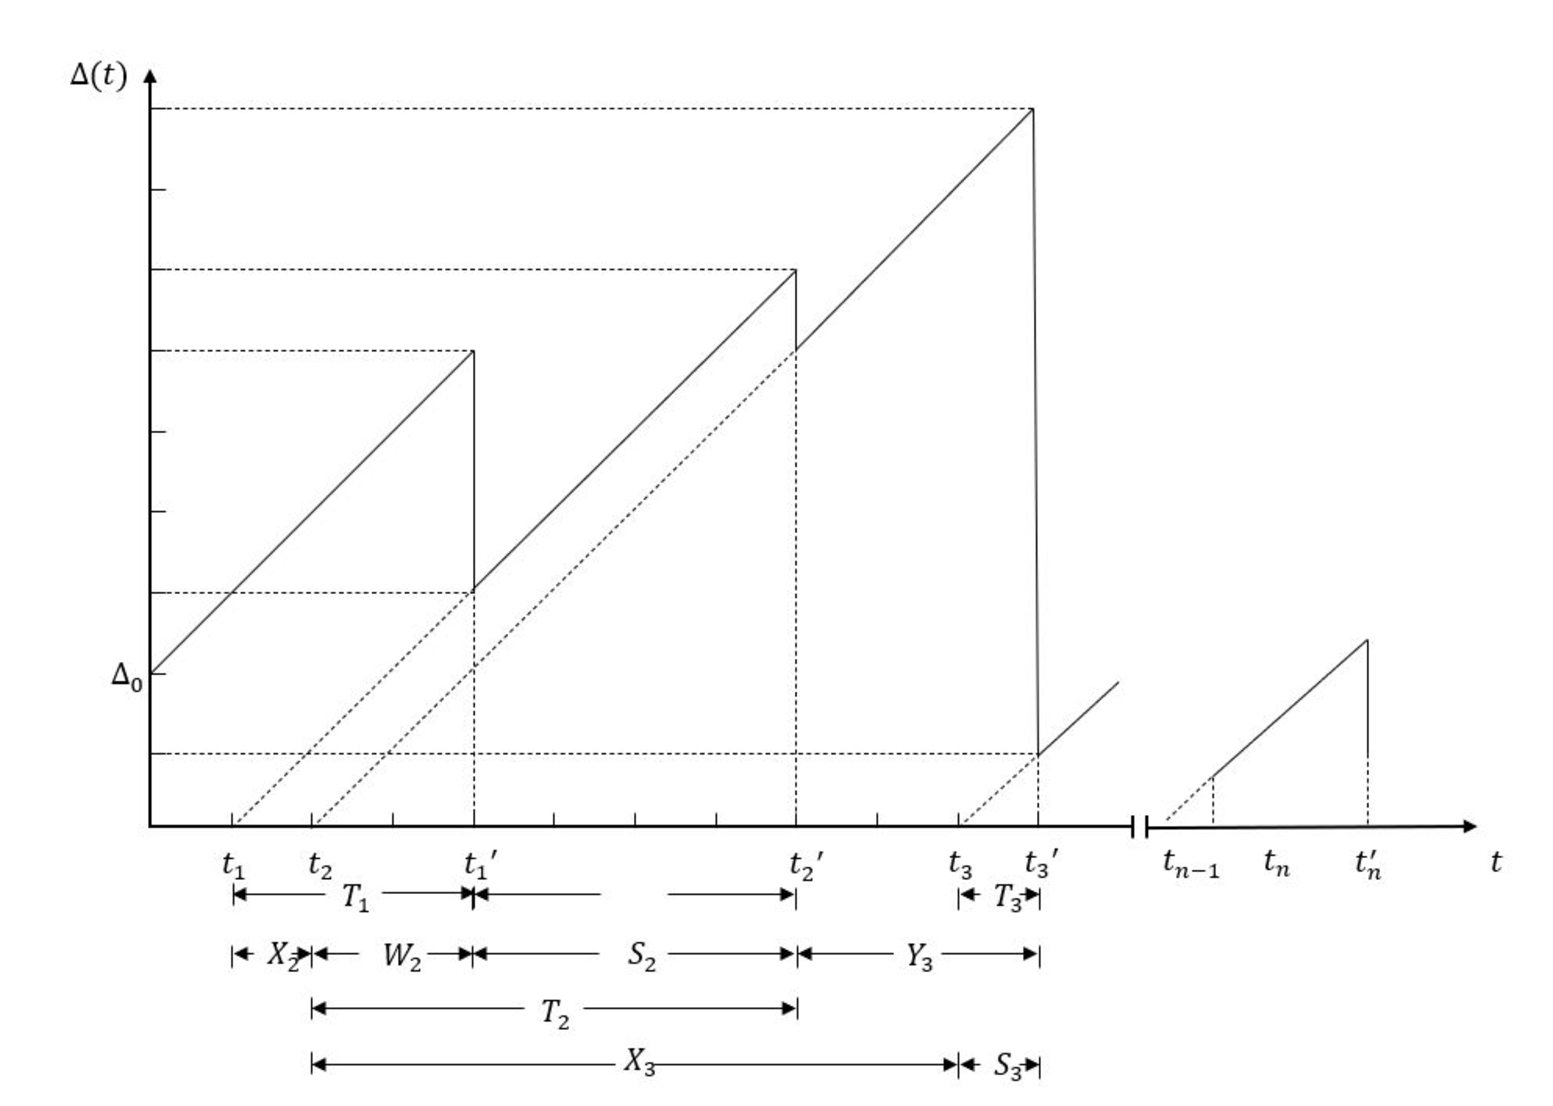
\includegraphics[width=0.8\textwidth]{figure/cp2/2.2.pdf}
    \caption{信息年龄变化趋势图}
    \label{fig:AoI_evolution}
\end{figure}

为了定量分析 AoI 的演化过程，我们对一些关键的系统随机变量进行定义。记$T_k$数据包更新的系统时间，$X_k$ 为第 $k$ 个数据包与第 $k-1$ 个数据包生成时刻之间的时间间隔，$S_k$ 为第 $k$ 个数据包在服务端的实际服务时间，$Y_k$ 为接收端成功收到第 $k-1$ 个与第 $k$ 个数据包之间的更新时间间隔。从图\ref{fig:AoI_evolution}可以发现，当数据包到达的间隔$X$较小，如$X_2<T_1$时，由于上一个包仍未完成传输，因此新数据包需在队列中进行等待，直到上一个包传输完成，因此两次更新的间隔完全取决于新包的服务时间，即$Y_2=S_2$。反之，若数据包的到达非常稀疏，比如$X_3>T_2$，当新包到来时，由于上一个包早已传输完毕且信道处于空闲状态，系统经历了一段无包可传的空窗期，所以更新间隔将被拉长为$Y_3=X_3+S_3-T_2$。因此，对于$Y_k$，我们可以总结出以下规律：
\begin{equation}
    Y_{k}=
\begin{cases}
S_{k}, & \text{if } X_{k} \leq T_{k-1} \\
X_{k} + S_{k} - T_{k-1}, & \text{if } X_{k} > T_{k-1}
\end{cases}
\end{equation}

\subsubsection{AoI的相关指标}

为了在后续章节中对等待 ALOHA 和等待 CSMA 等具体协议进行定量的理论评估，我们需要基于上述锯齿波形，推导出通用的计算公式。

\begin{enumerate}[wide]
    \item 平均AoI
    
    平均 AoI 用于衡量系统在长期运行平稳后的总体信息新鲜度，它是评估网络常规时效性的最核心指标。其数学本质是瞬时 AoI $\Delta(t)$ 在整个观测时间轴上的时间平均值：
    \begin{equation} \label{avg_AoI}
        \Delta = \lim_{T \to +\infty} \frac{1}{T} \int_{0}^{T} \Delta(t) dt
    \end{equation}

    \begin{figure}[h]
    \centering
    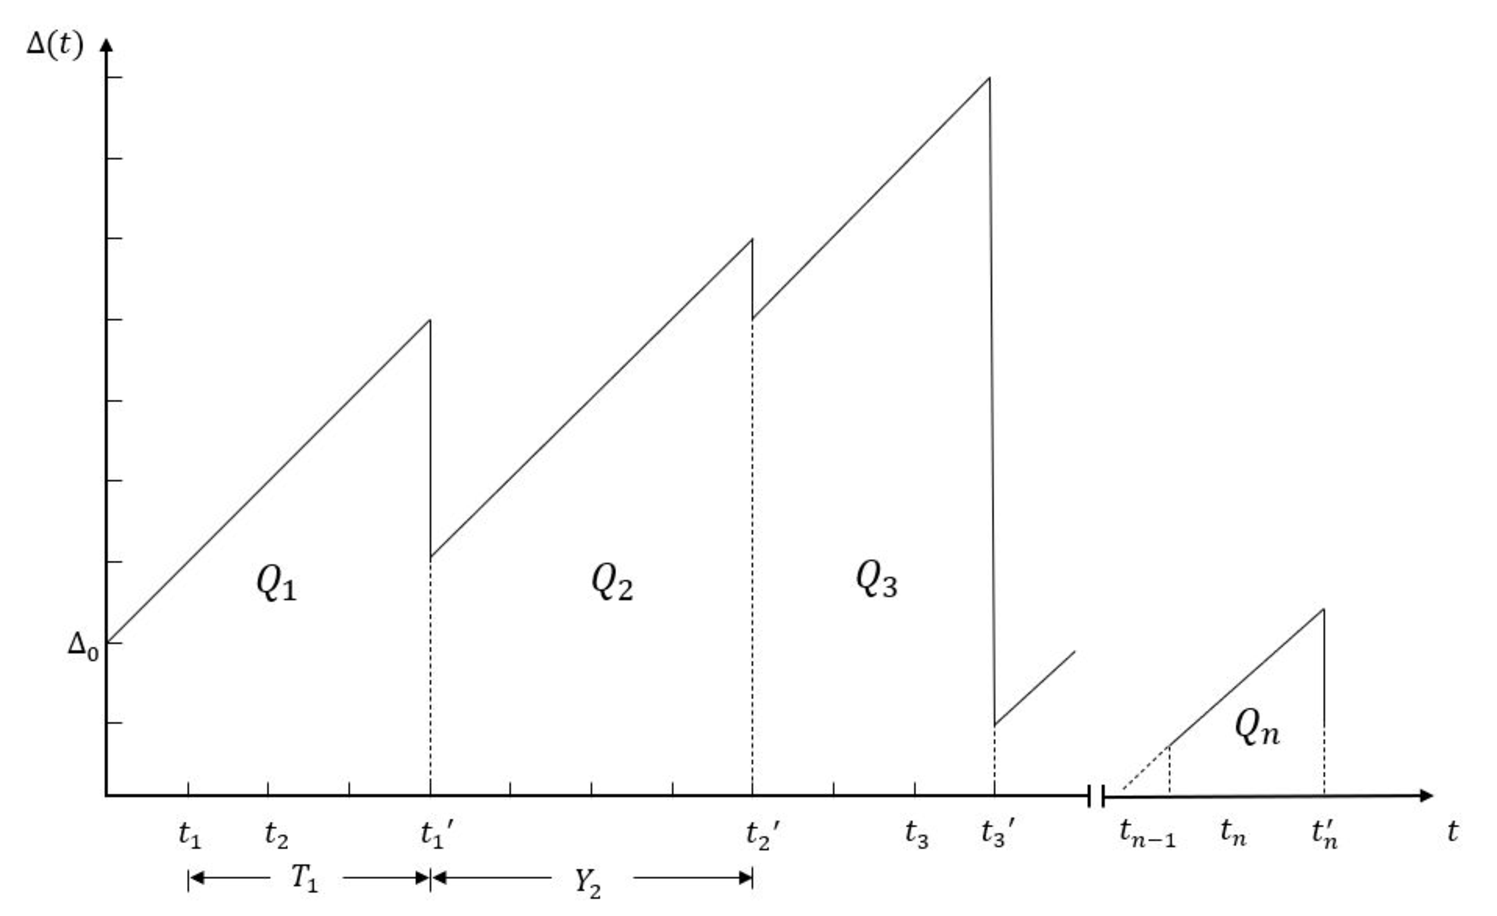
\includegraphics[width=0.8\textwidth]{figure/cp2/2.3.pdf}
    \caption{AoI曲线的面积分解示意图}
    \label{fig:AoI_evolution_mianjihuafen}
    \end{figure}

    为了求解这一连续积分，我们可以采用几何面积分解法。将总观测时间$T$划分为N个不重叠的更新区间，每个区间由两次连续的数据包接收时刻$t'_{n-1}$和$t'_n$确定。令$Q_n$为第$n$个区间内$\Delta(t)$曲线下方的面积，如图\ref{fig:AoI_evolution_mianjihuafen}所示，对梯形$Q_n$进行分析：
     \begin{itemize}
         \item 底边长度：$Y_n=t'_n-t'_{n-1}$；
         \item 左侧高度：在$t'_{n-1}$时刻，AoI刚完成重置，值为上一个包的系统时间，即$T_{n-1}$；
         \item 右侧高度：AoI随时间线性增长，直到$t'_n$时刻重置，此时高度为$T_{n-1}+Y_n$。
     \end{itemize}
     因此单个梯形$Q_n$的面积为：
     \begin{equation}
        \begin{aligned}
        Q_n &= \frac{1}{2} Y_n \big(T_{n-1} + (T_{n-1} + Y_n)\big) \\
        &= \frac{1}{2} Y_n \big(2T_{n-1} + Y_n\big) \\
        &= Y_n T_{n-1} + \frac{1}{2} Y_n^2
        \end{aligned}
     \end{equation}
     在总时间 $T$ 内，曲线下方的总面积是所有梯形面积的总和，因此平均 AoI 的公式可重写为：
     \begin{equation}\label{aoitoarea}
         \Delta =  \lim_{T \to +\infty} \frac{1}{T} \sum_{n=1}^{N} Q_n
     \end{equation}

     随着观测时间$T$的增加，数据包的总数$N$也趋于无穷，利用大数定理，我们可以将求和式的极限转化为离散随机变量的统计期望运算，即$\frac{1}{N} \sum Q_n \to E[Q]$以及$\frac{T}{N} \to E[Y]$，最后，我们得到了求解平均 AoI 的通用期望公式：
     \begin{equation}\label{cp2_avg_aoi}
         \Delta = \frac{E[Q]}{E[Y]} = \frac{E\left[Y_n T_{n-1} + \frac{1}{2} Y_n^2\right]}{E[Y]}=\frac{E[Y T] + \frac{1}{2} E[Y^2]}{E[Y]}
     \end{equation}
     该表达式具有极强的通用性。在后续的第三章和第四章中，无论具体的退避机制多么复杂，我们只需结合具体的系统模型，分别求解出该协议下的更新间隔期望 $E[Y]$、二阶矩 $E[Y^2]$ 以及交叉项期望 $E[Y T]$，即可代入此公式迅速获得平均 AoI 的闭式解。
    
    \item 峰值AoI
    
    与平均 AoI 关注系统的常态不同，峰值 AoI 旨在捕捉系统信息新鲜度在局部时刻的最差表现。它代表了接收端在迎来下一次状态刷新前夕，所忍受的最大信息陈旧度，即锯齿曲线在每次断崖式下降前所达到的尖峰值。令 $t_k$ 为第 $k$ 次成功接收的时刻，则第 $k$ 个峰值定义为：
    \begin{equation}
        \text{PA}_k = \lim_{t \to t_k^-} \Delta(t) = \Delta(t_k^-) = T_{k-1} + Y_k
    \end{equation}

    对于一些对极端延迟极其敏感且容错率极低的工业控制应用而言，掌握系统的最差新鲜度情况至关重要。为了评估系统的长期最差性能水平，我们通常计算所有峰值的统计均值，即平均峰值 AoI。基于大数定理，当样本峰值数量 $K \to +\infty$ 时，其时间平均收敛于期望值：
    \begin{equation}\label{avg_peak_aoi}
        \overline{\text{PA}} = \lim_{K \to +\infty} \frac{1}{K} \sum_{k=1}^{K} \text{PA}_k =  \lim_{K \to +\infty} \frac{1}{K} \sum_{k=1}^{K} (T_{k-1} + Y_k)
    \end{equation}
    假设系统处于遍历且平稳的工作状态，上式可被极大简化为各个随机变量期望的线性叠加：
    \begin{equation}
        \overline{\text{PA}} =  E[T] + E[Y]
    \end{equation}
    
    \item 信息年龄的违规概率
    
    尽管平均 AoI 和峰值 AoI 分别刻画了系统的总体面貌和局部极值，但在自动驾驶、无人机协同等严苛场景中，系统往往存在一条不可逾越的“安全红线”。只要信息陈旧度越过这条红线，系统就会面临崩溃的风险。因此，我们引入了信息年龄的违规概率：在系统漫长的运行周期中，AoI 超过某一预设的阈值 $\omega$ 的时间占比。其严格定义为：
    \begin{equation}
        \Pr\{\Delta > \omega\} = \lim_{T \to +\infty} \frac{1}{T} \int_{0}^{T} \mathbf{1}_{\{\Delta(t) > \omega\}} dt
    \end{equation}
    其中，$\mathbf{1}_{\{\Delta(t) > \omega\}}$为标准指示函数，当$\Delta(t) > \omega$时取值为1，反之取值为0。

    \begin{figure}[h]
    \centering
    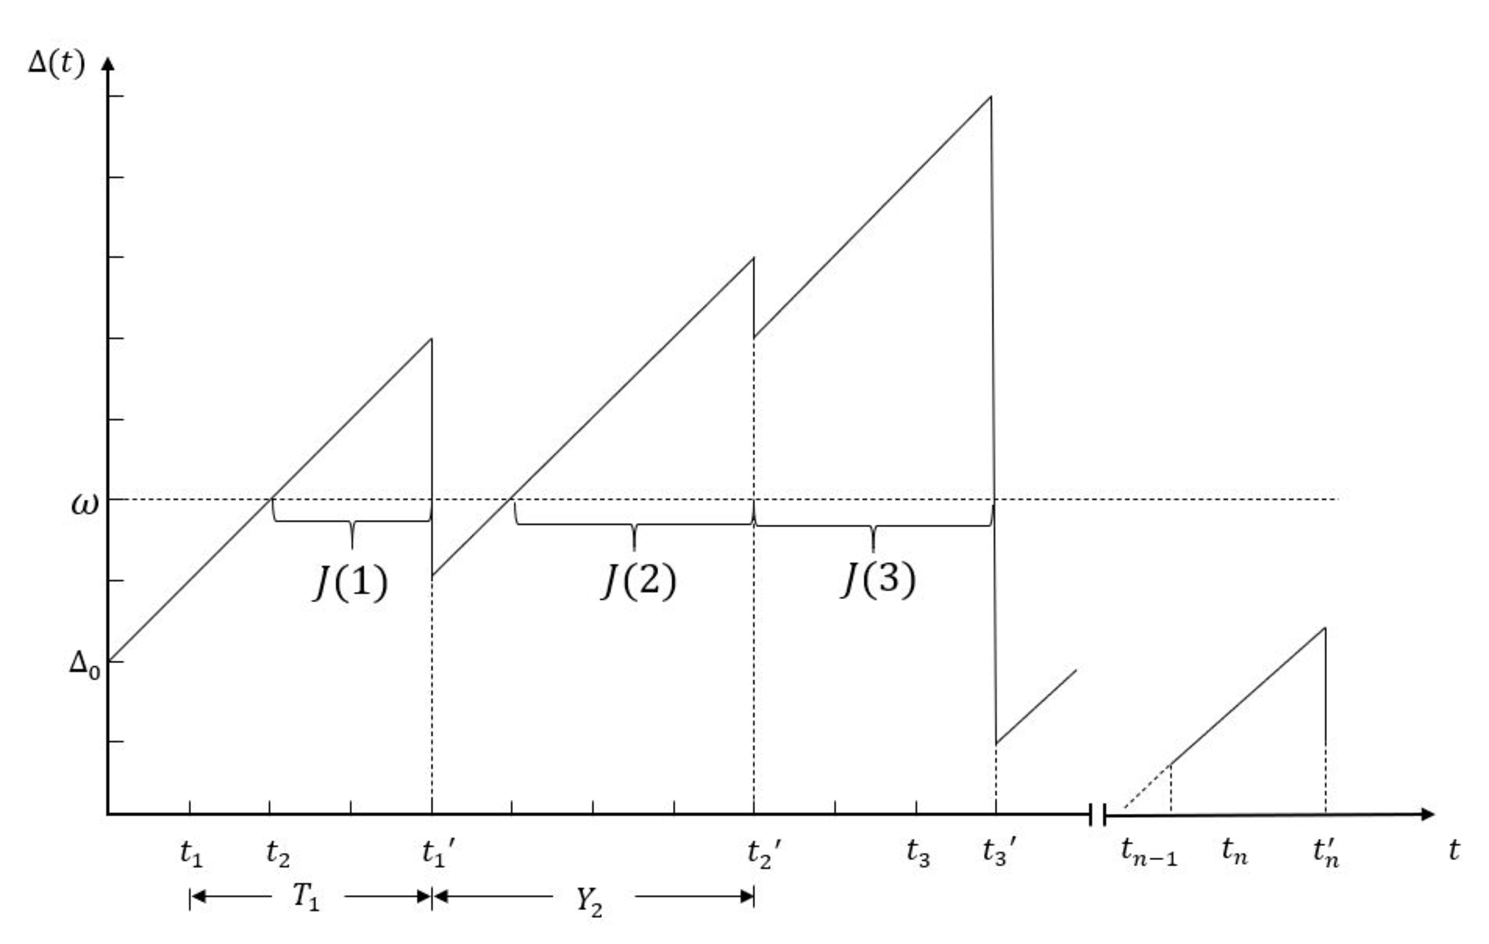
\includegraphics[width=0.8\textwidth]{figure/cp2/2.4.pdf}
    \caption{具有$\omega$限制的AoI演化图}
    \label{fig:AoI_evolution_with_limit}
    \end{figure}

    为了在离散的协议分析中计算这一连续概率，我们需要再次借助几何分解的思想 。我们定义 $J(k)$ 为第 $k$ 个更新周期，即区间 $[t'_{k-1}, t'_k]$内，AoI 曲线游离于安全阈值 $\omega$ 之上的持续时长，如图\ref{fig:AoI_evolution_with_limit}所示。观察演化曲线可以清晰地发现，在一个周期内，AoI 是单调递增的，只有当该周期的峰值 $\text{PA}_k$ 突破了阈值 $\omega$，系统才会发生违规事件。由于曲线斜率为 1，超出部分的垂直高度与其在水平时间轴上的投影长度严格相等，因此单次更新周期内的违规时长 $J(k)$ 可以通过下式计算：
    \begin{equation}\label{J_expression}
        J(k) = \max(0, PA(k) - \omega)
    \end{equation}
  
    按照与推导平均 AoI 完全一致的遍历性逻辑，假设在极长观测时间 $T$ 内系统完成了 $N$ 次数据包的更新，则总违规时间为 $\sum_{k=1}^{N}J(k)$。通过对式子进行变换，AoI 违规概率的通用计算闭式可推演为：
    \begin{equation}\label{cp2_aoi_violation_expression}
    \Pr\!\big(\Delta(t) > \omega\big) = \lim_{T \to +\infty} \frac{1}{T} \sum_{k=1}^{N} J(k) = \lim_{T \to +\infty} \frac{N}{T} \frac{1}{N} \sum_{k=1}^{N} J(k) = \frac{E[J]}{E[Y]}
    \end{equation}
\end{enumerate}

至此，我们分别建立了平均 AoI 与 AoI 违规概率的通用计算公式。在接下来的章节，我们会在具体的协议分析中利用这些公式，以此实现对不同协议时效性的定量评估与横向对比。

\subsection{马尔可夫链相关概述}
在后续的章节中，离散时间马尔可夫链（Discrete-time Markov chain, DTMC）是重要的理论分析工具，本节将系统地介绍它的相关理论。

\subsubsection{马尔可夫链的定义}
离散时间马尔可夫链是描述随机序列 $\{X_n : n=0, 1, 2, \dots\}$ 的一种数学模型。其核心特性是“无后效性”，即给定当前状态，未来演化与过去无关。具体地，设状态空间为可数集合 $S$，若对任意 $n$ 及任意 $i_0, i_1, \dots, i_{n+1} \in S$ 有：
\begin{equation}
    \begin{split}
        &\Pr(X_{n+1}=i_{n+1} \mid X_n=i_n, X_{n-1}=i_{n-1}, \dots, X_0=i_0) \\
        &\quad = \Pr(X_{n+1}=i_{n+1} \mid X_n=i_n)
    \end{split}
\end{equation}
则称 $\{X_n\}$ 为马尔可夫链。

\subsubsection{转移概率矩阵}
为了定量刻画马尔可夫链在不同状态之间的演化规律，我们引入一步转移概率。假设可数集合 $S$ 包含 $N$ 个可能的状态，记为 $\{S_1, S_2, \dots, S_N\}$。定义 $p_{ij}$ 为系统从当前状态 $i$ 经过一个离散时间步后，一步转移到状态 $j$ 的概率。显然，该概率必须满足非负性，即 $0 \le p_{ij} \le 1$。将系统中所有可能的状态转移概率按行与列排列，即可构建出刻画系统全貌的转移概率矩阵 $P$。该矩阵是一个 $N \times N$ 的方阵：
\begin{equation}
    P = \begin{bmatrix}
        p_{11} & p_{12} & \cdots & p_{1n} \\
        p_{21} & p_{22} & \cdots & p_{2n} \\
        \vdots & \vdots & \ddots & \vdots \\
        p_{n1} & p_{n2} & \cdots & p_{nn}
    \end{bmatrix}
\end{equation}
作为描述完备概率空间的随机矩阵，转移概率矩阵 $P$ 具有一个极其重要的数学性质：即系统从任意状态 $i$ 出发，在下一时刻必然转移到状态空间 $S$ 中的某一个状态。因此，矩阵 $P$ 中每一行的元素之和必须严格等于 1，即 $\sum_{j=1}^{N} p_{ij} = 1, \forall i \in S$。

\subsubsection{马尔可夫链的核心性质}
\begin{enumerate}[wide]
    \item \textbf{齐次性}：马尔可夫链的转移概率不随时间而变化。对于任意时刻 $t$ 和状态 $i, j$，一步转移概率满足：
    \begin{equation}
        P(X_{t+1}=j \mid X_t=i) = P(X_2=j \mid X_1=i) = p_{ij}
    \end{equation}
    即转移概率仅与“当前状态”和“目标状态 $j$”有关，与时刻 $t$ 无关。

    \item \textbf{可达性}：从状态 $i$ 出发，经过有限步转移能到达状态 $j$，就称 $j$ 从 $i$ 可达。

    \item \textbf{不可约性}：如果马尔可夫链中任意两个状态都相互可达，则称马尔可夫链具有不可约性。

    \item \textbf{周期性}：对于状态 $i$，定义其周期 $d(i)$ 为：
    \begin{equation}
        d(i) = \gcd\{n \ge 1 : P^{(n)}(i,i) > 0\}
    \end{equation}
    其中，$\gcd$ 表示最大公约数，$P^{(n)}(i,i)$ 表示从状态 $i$ 出发，经过 $n$ 步回到 $i$ 的概率。若 $d(i)=1$，状态为非周期；若 $d(i)>1$，则状态的周期为 $d(i)$。对于有不可约性的马尔可夫链，其所有状态的周期都相同。

    \item \textbf{遍历性}：对于马尔可夫链，如果它同时具有有限个状态、齐次性、不可约性和非周期性，那么我们称这条马尔可夫链具有遍历性。满足遍历性的马尔可夫链，无论其初始状态是什么，随着时间的推移，处于每个状态的概率最终都会收敛到一个固定值，且这个值是唯一的。
\end{enumerate}

\subsubsection{马尔可夫链的稳态分布}
如果一条具有遍历性的马尔可夫链运行足够长的时间（$t \to \infty$），那么其处于每个状态的概率将不再变化，这个固定的概率分布就是稳态分布。设 $\boldsymbol{\pi} = [\pi_1, \pi_2, \dots, \pi_n]$ 为稳态概率向量，$\pi_i$表示长期处于状态$i$的概率，其满足两个核心条件：
\begin{equation}
    \begin{cases}
        \boldsymbol{\pi} P = \boldsymbol{\pi} & \text{(概率守恒：转移后分布不变)} \\
        \sum_{i=1}^{n} \pi_i = 1 & \text{(归一化：所有状态概率和为1)}
    \end{cases}
\end{equation}
在系统达到稳态时，对于任意一个状态 $j$，系统在单位时间内离开状态 $j$ 的概率总流量，必然严格等于从其他所有状态转移并进入状态 $j$ 的概率总流量。




